\documentclass[14pt]{extbook}
\usepackage{multicol, enumerate, enumitem, hyperref, color, soul, setspace, parskip, fancyhdr} %General Packages
\usepackage{amssymb, amsthm, amsmath, bbm, latexsym, units, mathtools} %Math Packages
\everymath{\displaystyle} %All math in Display Style
% Packages with additional options
\usepackage[headsep=0.5cm,headheight=12pt, left=1 in,right= 1 in,top= 1 in,bottom= 1 in]{geometry}
\usepackage[usenames,dvipsnames]{xcolor}
\usepackage{dashrule}  % Package to use the command below to create lines between items
\newcommand{\litem}[1]{\item#1\hspace*{-1cm}\rule{\textwidth}{0.4pt}}
\pagestyle{fancy}
\lhead{Progress Quiz 9}
\chead{}
\rhead{Version C}
\lfoot{8590-6105}
\cfoot{}
\rfoot{Fall 2020}
\begin{document}

\begin{enumerate}
\litem{
Solve the equation below. Then, choose the interval that contains the solution.\[ -13(-12x + 6) = -14(-9x -10) \]\begin{enumerate}[label=\Alph*.]
\item \( x \in [6.5, 7.9] \)
\item \( x \in [-3.4, -1.3] \)
\item \( x \in [-1.3, 1] \)
\item \( x \in [1.1, 2.5] \)
\item \( \text{There are no real solutions.} \)

\end{enumerate} }
\litem{
Solve the linear equation below. Then, choose the interval that contains the solution.\[ \frac{3x + 3}{2} - \frac{-4x + 3}{7} = \frac{9x -4}{4} \]\begin{enumerate}[label=\Alph*.]
\item \( x \in [19.4, 23.4] \)
\item \( x \in [0.04, 4.04] \)
\item \( x \in [10.6, 13.6] \)
\item \( x \in [15.4, 17.4] \)
\item \( \text{There are no real solutions.} \)

\end{enumerate} }
\litem{
Solve the equation below. Then, choose the interval that contains the solution.\[ -17(2x + 19) = -16(18x + 10) \]\begin{enumerate}[label=\Alph*.]
\item \( x \in [1.33, 2.82] \)
\item \( x \in [-1.81, -1.36] \)
\item \( x \in [-2.13, -1.86] \)
\item \( x \in [-0.41, 0.7] \)
\item \( \text{There are no real solutions.} \)

\end{enumerate} }
\litem{
Write the equation of the line in the graph below in Standard form $Ax+By=C$. Then, choose the intervals that contain $A, B, \text{ and } C$.
\begin{center}
    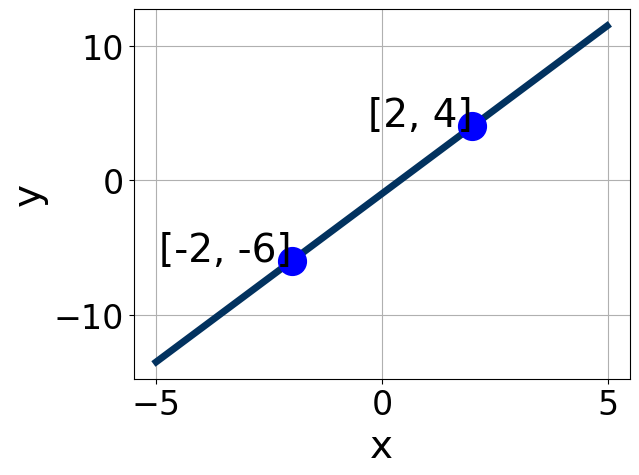
\includegraphics[width=0.5\textwidth]{../Figures/linearGraphToStandardCopyC.png}
\end{center}
\begin{enumerate}[label=\Alph*.]
\item \( A \in [-4.67, 2.33], \hspace{3mm} B \in [0.55, 1.01], \text{ and } \hspace{3mm} C \in [-3, 1] \)
\item \( A \in [-7, -2], \hspace{3mm} B \in [2.05, 4.35], \text{ and } \hspace{3mm} C \in [-3, 1] \)
\item \( A \in [-4.67, 2.33], \hspace{3mm} B \in [-2.07, 0.04], \text{ and } \hspace{3mm} C \in [-3, 1] \)
\item \( A \in [5, 11], \hspace{3mm} B \in [-3.85, -2.46], \text{ and } \hspace{3mm} C \in [-3, 1] \)
\item \( A \in [5, 11], \hspace{3mm} B \in [2.05, 4.35], \text{ and } \hspace{3mm} C \in [-3, 1] \)

\end{enumerate} }
\litem{
Solve the linear equation below. Then, choose the interval that contains the solution.\[ \frac{-3x + 5}{8} - \frac{-9x -4}{7} = \frac{4x + 7}{4} \]\begin{enumerate}[label=\Alph*.]
\item \( x \in [21.4, 23.4] \)
\item \( x \in [-5.72, 3.28] \)
\item \( x \in [-6.2, -1.2] \)
\item \( x \in [-20, -17] \)
\item \( \text{There are no real solutions.} \)

\end{enumerate} }
\litem{
Find the equation of the line described below. Write the linear equation as $ y=mx+b $ and choose the intervals that contain $m$ and $b$.\[ \text{Parallel to } 9 x + 8 y = 4 \text{ and passing through the point } (-4, -6). \]\begin{enumerate}[label=\Alph*.]
\item \( m \in [-1.14, -0.97] \hspace*{3mm} b \in [-11.02, -10.08] \)
\item \( m \in [1.03, 1.13] \hspace*{3mm} b \in [-1.54, -1.23] \)
\item \( m \in [-0.92, -0.85] \hspace*{3mm} b \in [-11.02, -10.08] \)
\item \( m \in [-1.14, -0.97] \hspace*{3mm} b \in [10.34, 10.79] \)
\item \( m \in [-1.14, -0.97] \hspace*{3mm} b \in [-2.37, -1.85] \)

\end{enumerate} }
\litem{
Find the equation of the line described below. Write the linear equation as $ y=mx+b $ and choose the intervals that contain $m$ and $b$.\[ \text{Parallel to } 4 x - 3 y = 13 \text{ and passing through the point } (-7, 10). \]\begin{enumerate}[label=\Alph*.]
\item \( m \in [0.94, 1.92] \hspace*{3mm} b \in [17.4, 20.7] \)
\item \( m \in [-1.85, -1.23] \hspace*{3mm} b \in [-0.4, 3] \)
\item \( m \in [0.94, 1.92] \hspace*{3mm} b \in [15.9, 18.8] \)
\item \( m \in [-0.24, 1.22] \hspace*{3mm} b \in [17.4, 20.7] \)
\item \( m \in [0.94, 1.92] \hspace*{3mm} b \in [-20.1, -18.2] \)

\end{enumerate} }
\litem{
Write the equation of the line in the graph below in Standard form $Ax+By=C$. Then, choose the intervals that contain $A, B, \text{ and } C$.
\begin{center}
    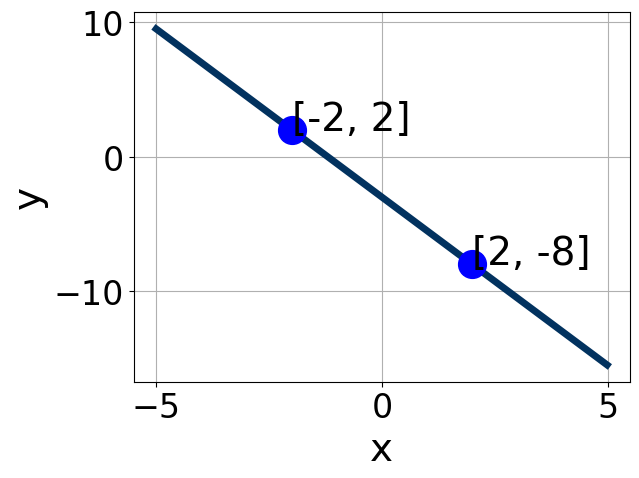
\includegraphics[width=0.5\textwidth]{../Figures/linearGraphToStandardC.png}
\end{center}
\begin{enumerate}[label=\Alph*.]
\item \( A \in [-2.5, 3.5], \hspace{3mm} B \in [-1.23, 0.17], \text{ and } \hspace{3mm} C \in [1.4, 4.6] \)
\item \( A \in [-2.5, 3.5], \hspace{3mm} B \in [0.76, 1.01], \text{ and } \hspace{3mm} C \in [-4.8, -1.8] \)
\item \( A \in [5, 6], \hspace{3mm} B \in [1.94, 2.18], \text{ and } \hspace{3mm} C \in [-8.4, -4.1] \)
\item \( A \in [5, 6], \hspace{3mm} B \in [-2.09, -1.77], \text{ and } \hspace{3mm} C \in [4.6, 7.2] \)
\item \( A \in [-6, -2], \hspace{3mm} B \in [-2.09, -1.77], \text{ and } \hspace{3mm} C \in [4.6, 7.2] \)

\end{enumerate} }
\litem{
First, find the equation of the line containing the two points below. Then, write the equation as $ y=mx+b $ and choose the intervals that contain $m$ and $b$.\[ (3, 8) \text{ and } (7, -10) \]\begin{enumerate}[label=\Alph*.]
\item \( m \in [3.5, 8.5] \hspace*{3mm} b \in [-46.5, -38.5] \)
\item \( m \in [-6.5, -2.5] \hspace*{3mm} b \in [3, 8] \)
\item \( m \in [-6.5, -2.5] \hspace*{3mm} b \in [-25.5, -19.5] \)
\item \( m \in [-6.5, -2.5] \hspace*{3mm} b \in [18.5, 24.5] \)
\item \( m \in [-6.5, -2.5] \hspace*{3mm} b \in [-17, -15] \)

\end{enumerate} }
\litem{
First, find the equation of the line containing the two points below. Then, write the equation as $ y=mx+b $ and choose the intervals that contain $m$ and $b$.\[ (11, -5) \text{ and } (6, -7) \]\begin{enumerate}[label=\Alph*.]
\item \( m \in [0.1, 2.2] \hspace*{3mm} b \in [-15, -10] \)
\item \( m \in [0.1, 2.2] \hspace*{3mm} b \in [-9.4, -5.4] \)
\item \( m \in [0.1, 2.2] \hspace*{3mm} b \in [-20, -15] \)
\item \( m \in [-1.4, 0.2] \hspace*{3mm} b \in [-5.6, 1.4] \)
\item \( m \in [0.1, 2.2] \hspace*{3mm} b \in [5.4, 13.4] \)

\end{enumerate} }
\end{enumerate}

\end{document}